\section{Aufbau}
\label{sec:Aufbau}

\begin{figure}
\centering
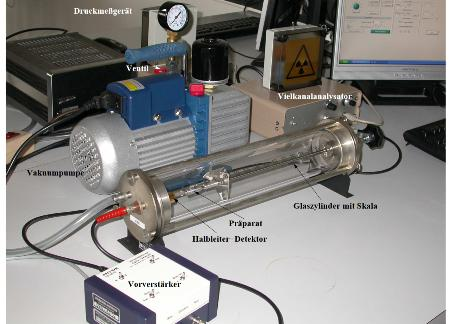
\includegraphics[scale=0.6]{content/images/aufbau.jpg}
\caption{Aufbau zur Bestimmung der Reichweite von $\alpha$-Strahlung\cite{V701}}
\label{fig:aufbau}
\end{figure}

\noindent Das Experiment bestehend aus einem Glaszylinder mit Vakuumpumpe, einem Am-Präparat und einem Halbleiter-Sperrschichtzähler wird gemäß Abbildung \ref{fig:aufbau} mit einem Vorverstärker und einem Vielkanalanalysator gekoppelt, der an einen Computer angeschlossen ist.
Sowohl Detektor als auch Präparat können innerhalb des Glaszylinders verschoben werden.
